\chapter{Spatial Domain: \refmod}
\label{ch:ref-mod}

It was Xenakis' goal for the curved surfaces of the Philips Pavilion
to reduce the sonic contribution of sound reflections as much as
possible.\cite{philips1958} He knew that reflections and the resulting
comb filtering could impair intelligibility and localization of music
and sounds. The pavilion was to have hundreds of loudspeaker, and
large concave surfaces like the ones on the inside of the pavilion can
have a focussing effect on acoustic reflections, resulting in severe
filtering and phase cancellations.\cite{Vercammen2008} If Xenakis had
been able to model the reflections and compose them directly into the
piece, what would the tools be like, and how would his architectural
spaces be different? The Xenakis inspired \refmod is an abstract
software tool for experimenting with architectural acoustic lenses. It
is intended more as an experiment for architectural or musical
brainstorming than as a simulation for analysis of sound
propagation. For example:
\begin{enumerate}
\item It illustrates sound projection in only two dimensions.
\item It is frequency independent. Real sufaces reflect only
  wavelengths much smaller than the size of the
  reflector.\cite{Zhixin2005} 
\item Diffraction is ignored. 
\item Acoustic sounds waves of higher frequencies propagate more
  directionally than lower frequencies. This property is ignored.
% \item The acoustic reflections from, and acoustic diffraction around a
%   real object are dependent on the materials and obstacles behind
%   or adjacent the reflecting surface.\cite{Howard2006} This effect is
%   also not taken modeled by the \refmod.
\end{enumerate}

\section{Implementation}
\label{sec:refmod-implementation}
The \refmod was implemented as a web app using the HTML5
Paper.js\sidenote{\url{http://paperjs.org/}} vector graphics
library. \marginnote{Try \refmod online at\\
\noindent \url{http://web.media.mit.edu/~holbrow/mas/reflections/}}
 Click and drag on any black dot to move the
object. Black dots connected by grey lines are handles that
re-orient (instead of move) objects. On reflection surfaces, the handles
adjust the angle and shape of the surface curve. Handles connected to
sound sources adjust the angle and length of the sound beams. 
\begin{figure}[h]
% http://web.media.mit.edu/~holbrow/mas/reflections/?q=%7B%22mirrors%22%3A%5B%5B%22Path%22%2C%7B%22applyMatrix%22%3Atrue%2C%22segments%22%3A%5B%5B%5B330%2C60%5D%2C%5B0%2C0%5D%2C%5B-239%2C185%5D%5D%2C%5B319%2C424%5D%5D%2C%22strokeColor%22%3A%5B0%2C0%2C0%5D%2C%22strokeWidth%22%3A2%7D%5D%2C%5B%22Path%22%2C%7B%22applyMatrix%22%3Atrue%2C%22segments%22%3A%5B%5B%5B1035%2C436%5D%2C%5B0%2C0%5D%2C%5B-135%2C113%5D%5D%2C%5B1123%2C534%5D%5D%2C%22strokeColor%22%3A%5B0%2C0%2C0%5D%2C%22strokeWidth%22%3A2%7D%5D%5D%2C%22sounds%22%3A%5B%5B%22Path%22%2C%7B%22applyMatrix%22%3Atrue%2C%22segments%22%3A%5B%5B1047%2C123%5D%2C%5B1048%2C145%5D%5D%2C%22strokeColor%22%3A%5B0.6%2C0.6%2C0.6902%5D%7D%5D%2C%5B%22Path%22%2C%7B%22applyMatrix%22%3Atrue%2C%22segments%22%3A%5B%5B411%2C176%5D%2C%5B480%2C136%5D%5D%2C%22strokeColor%22%3A%5B0.6%2C0.6%2C0.6902%5D%7D%5D%5D%7D
  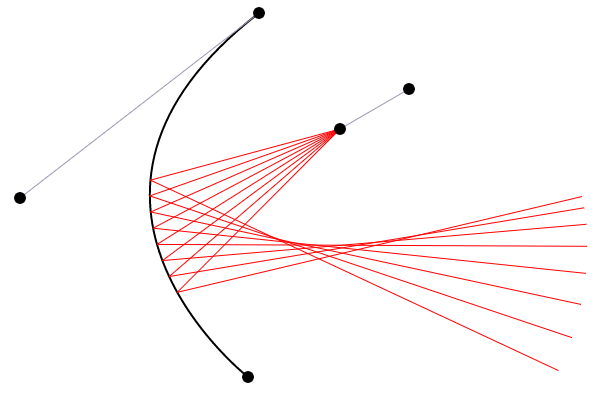
\includegraphics[width=\linewidth]{refmod/1.png}
  \caption[]{\refmod user interface.}
  \label{fig:refmod-simple}
\end{figure}

\section{\refmod Architectural Example}
\label{sec:refmod-user-interf}

Assume we are creating the floor plan for a new architectural space
and accompanying electronic music performance. The music piece
incorporates spatial component in the style of \textit{SOUND=SPACE} by
Rolf Gehlhaar: Our audience moves through the performance space, and
as they move, the sound changes, making the music experience unique to
every visitor. We would like to use acoustic reflections to manipulate
the sound in space, and such that at certain points the sound is
focussed on the lister. When we hear an acoustic sound reflection off
a concave surface, the sound can arrive at our ears in two possible
states:
\begin{enumerate}
\item The path of the sound from the source to the reflecting surface
  to our ears is equidistant for each point on the reflecting
  surface. Ignoring any direct sound, the reflection arrives in phase,
  and the surface acts as acoustic amplifier of the reflection.
\item The path of the sound from the source to the reflecting surface
  to our ears is slightly different for each point on the surface. All
  the reflections arrive out of phase with each other.
\end{enumerate}
We can use the this tool to prototype potential layouts and gain some
intuition about where our focal points. The curved black line in the
user interface (figure~\ref{fig:refmod-simple}) represents a
reflective surface. The black dot with emanating red lines represents
a sound source, and the sound propagation.  Each red line emanating
from a sound source is the same length, no matter how many times it
has been reflected. If it is possible to adjust the length of the red
lines such that each one ends at the same spot, it shows that
reflections will arrive at that spot in
phase. Figures~\ref{fig:refmod-bad-focus}
and~\ref{fig:refmod-good-focus} show how we can adjust the curve of a
surface to focus reflections on a point.

\begin{figure}[]
% http://web.media.mit.edu/~holbrow/mas/reflections/?q=%7B%22mirrors%22%3A%5B%5B%22Path%22%2C%7B%22applyMatrix%22%3Atrue%2C%22segments%22%3A%5B%5B%5B513%2C318%5D%2C%5B0%2C0%5D%2C%5B-218%2C117%5D%5D%2C%5B192%2C241%5D%5D%2C%22strokeColor%22%3A%5B0%2C0%2C0%5D%2C%22strokeWidth%22%3A2%7D%5D%2C%5B%22Path%22%2C%7B%22applyMatrix%22%3Atrue%2C%22segments%22%3A%5B%5B%5B1035%2C436%5D%2C%5B0%2C0%5D%2C%5B-135%2C113%5D%5D%2C%5B1123%2C534%5D%5D%2C%22strokeColor%22%3A%5B0%2C0%2C0%5D%2C%22strokeWidth%22%3A2%7D%5D%5D%2C%22sounds%22%3A%5B%5B%22Path%22%2C%7B%22applyMatrix%22%3Atrue%2C%22segments%22%3A%5B%5B1047%2C123%5D%2C%5B1048%2C145%5D%5D%2C%22strokeColor%22%3A%5B0.6%2C0.6%2C0.6902%5D%7D%5D%2C%5B%22Path%22%2C%7B%22applyMatrix%22%3Atrue%2C%22segments%22%3A%5B%5B220%2C202%5D%2C%5B177%2C150%5D%5D%2C%22strokeColor%22%3A%5B0.6%2C0.6%2C0.6902%5D%7D%5D%5D%7D
  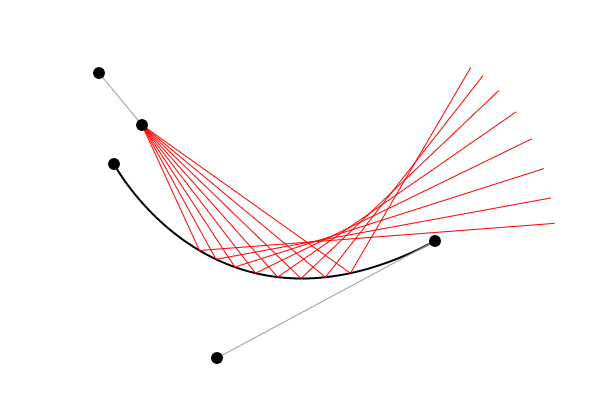
\includegraphics[width=\linewidth]{refmod/out-of-focus.png}
  \caption[]{Reflections from a $30\degree$ loudspeaker arriving out of phase.}
  \label{fig:refmod-bad-focus}
\end{figure}

\begin{figure}[]
%http://web.media.mit.edu/~holbrow/mas/reflections/?q=%7B%22mirrors%22%3A%5B%5B%22Path%22%2C%7B%22applyMatrix%22%3Atrue%2C%22segments%22%3A%5B%5B%5B525%2C318%5D%2C%5B0%2C0%5D%2C%5B-251%2C68%5D%5D%2C%5B180%2C242%5D%5D%2C%22strokeColor%22%3A%5B0%2C0%2C0%5D%2C%22strokeWidth%22%3A2%7D%5D%2C%5B%22Path%22%2C%7B%22applyMatrix%22%3Atrue%2C%22segments%22%3A%5B%5B%5B1035%2C436%5D%2C%5B0%2C0%5D%2C%5B-135%2C113%5D%5D%2C%5B1123%2C534%5D%5D%2C%22strokeColor%22%3A%5B0%2C0%2C0%5D%2C%22strokeWidth%22%3A2%7D%5D%5D%2C%22sounds%22%3A%5B%5B%22Path%22%2C%7B%22applyMatrix%22%3Atrue%2C%22segments%22%3A%5B%5B1047%2C123%5D%2C%5B1048%2C145%5D%5D%2C%22strokeColor%22%3A%5B0.6%2C0.6%2C0.6902%5D%7D%5D%2C%5B%22Path%22%2C%7B%22applyMatrix%22%3Atrue%2C%22segments%22%3A%5B%5B220%2C202%5D%2C%5B179%2C145%5D%5D%2C%22strokeColor%22%3A%5B0.6%2C0.6%2C0.6902%5D%7D%5D%5D%7D
  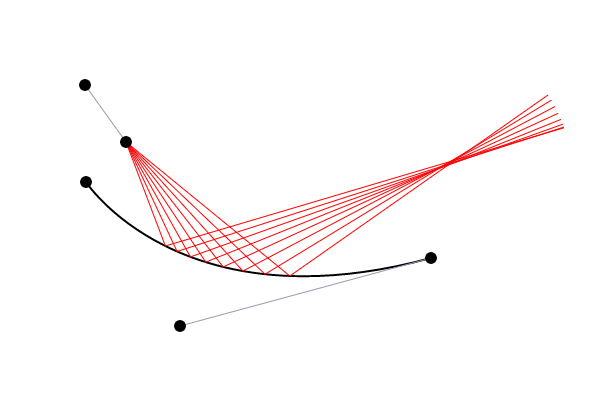
\includegraphics[width=\linewidth]{refmod/in-focus.png}
  \caption[]{By adjusting the curvature of the reflective surface, we
    can focus the audio reflections.}
  \label{fig:refmod-good-focus}
\end{figure}

\begin{figure}[]
%http://web.media.mit.edu/~holbrow/mas/reflections/?q=%7B%22mirrors%22%3A%5B%5B%22Path%22%2C%7B%22applyMatrix%22%3Atrue%2C%22segments%22%3A%5B%5B%5B169%2C416%5D%2C%5B0%2C0%5D%2C%5B405%2C234%5D%5D%2C%5B1178%2C571%5D%5D%2C%22strokeColor%22%3A%5B0%2C0%2C0%5D%2C%22strokeWidth%22%3A2%7D%5D%2C%5B%22Path%22%2C%7B%22applyMatrix%22%3Atrue%2C%22segments%22%3A%5B%5B%5B406%2C321%5D%2C%5B0%2C0%5D%2C%5B135%2C-41%5D%5D%2C%5B651%2C367%5D%5D%2C%22strokeColor%22%3A%5B0%2C0%2C0%5D%2C%22strokeWidth%22%3A2%7D%5D%5D%2C%22sounds%22%3A%5B%5B%22Path%22%2C%7B%22applyMatrix%22%3Atrue%2C%22segments%22%3A%5B%5B431%2C834%5D%2C%5B541%2C796%5D%5D%2C%22strokeColor%22%3A%5B0.6%2C0.6%2C0.6902%5D%7D%5D%2C%5B%22Path%22%2C%7B%22applyMatrix%22%3Atrue%2C%22segments%22%3A%5B%5B278%2C367%5D%2C%5B227%2C266%5D%5D%2C%22strokeColor%22%3A%5B0.6%2C0.6%2C0.6902%5D%7D%5D%5D%7D
  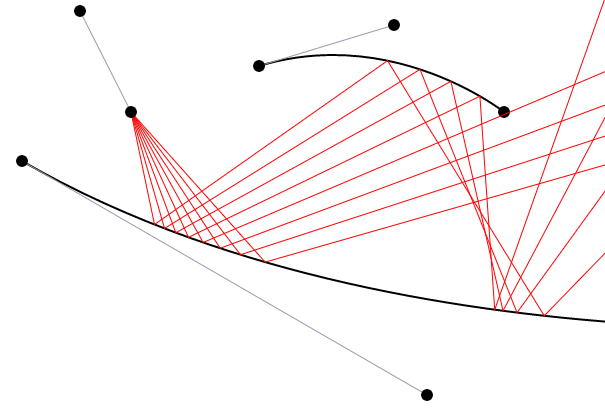
\includegraphics[width=\linewidth]{refmod/music.png}
  \caption[]{A musical composition. The red emanating lines can also
    be thought of as stochastic pitch swarms, similar to those Xenakis
    wrote for Metastasis in 1954 (figure~\ref{fig:metastasis}).}
  \label{fig:refmod-music}
\end{figure}


\begin{figure*}[]
  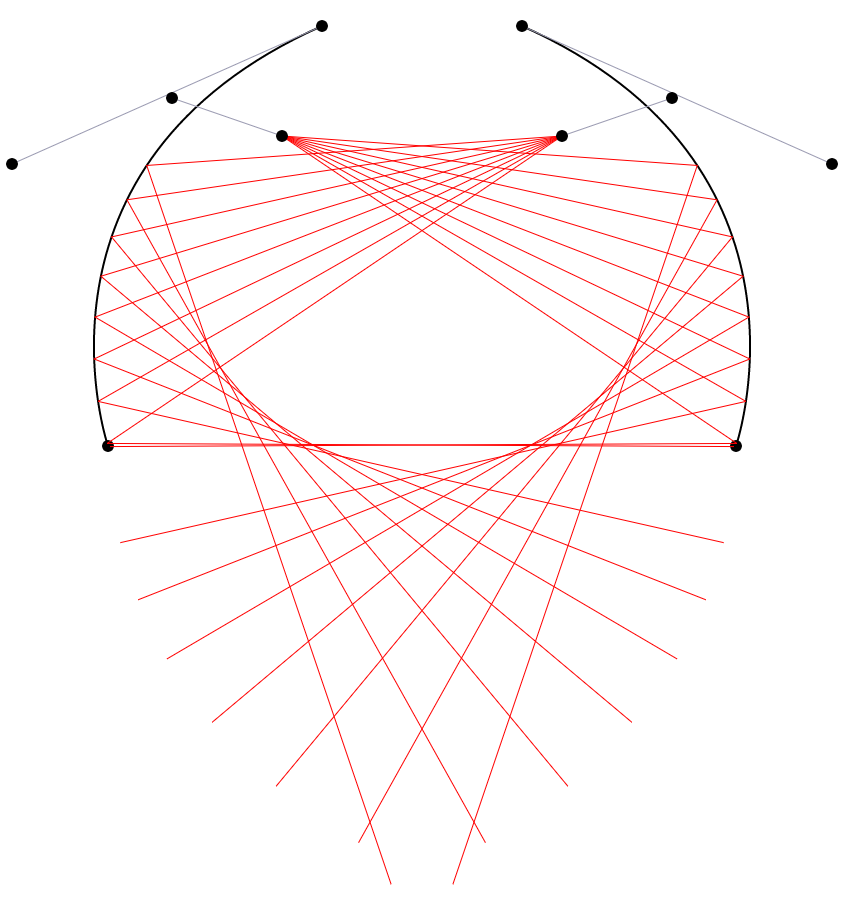
\includegraphics[width=\linewidth]{refmod/refmod.png}
  \caption[]{The \refmod.}
  \label{fig:refmod-full}
\end{figure*}


%%% Local Variables:
%%% mode: latex
%%% TeX-master: "CharlesHolbrow_MAS_Thesis"
%%% End:
